% !TEX root = ../Hamiltonian_of_mean_force.tex
\section{Generating-function structure of the influence operator\label{sec:generating_function}}

\subsection{Quenched propagator and Gaussian resummation\label{subsec:gaussian_resum}}

The starting point is the quenched propagator introduced in Sec.~\ref{sec:hmf}. In the imaginary-time
interaction picture with respect to $H_Q$, the unnormalised reduced equilibrium operator takes the form
\begin{equation}
    \begin{split}
        \bar\rho_Q(\beta)
        & = e^{-\beta H_Q}\,\langle W_\xi(\beta)\rangle_\xi, \\
        W_\xi(\beta)
        & \equiv \mathcal{T}_\tau\exp\!\left[-\int_0^\beta\!d\tau\,\xi(\tau)\,\tilde f(\tau)\right],
    \end{split}
    \label{eq:Wxi_rhobar_def}
\end{equation}
where $\tilde f(\tau)=e^{\tau H_Q}fe^{-\tau H_Q}$ and the noise covariance is
$\langle\xi(\tau)\xi(\tau')\rangle_\xi = K(\tau-\tau')$.

Because the bath is Gaussian, only the second cumulant of $\xi$ is non-vanishing. Time-ordering
introduces a non-trivial operator structure, but the key identity---proved in
Appendix~\ref{app:gaussian_averaging}---is that the Wick resummation of all pairings exponentiates
exactly:
\begin{equation}
    \langle W_\xi(\beta)\rangle_\xi
    = \exp\!\left[\frac{1}{2}\int_0^\beta\!d\tau\int_0^\beta\!d\tau'\,
      K(\tau-\tau')\,\mathcal{T}_\tau\!\big[\tilde f(\tau)\tilde f(\tau')\big]\right].
    \label{eq:Wbar_cumulant}
\end{equation}
The proof is a direct application of Wick's theorem to the Dyson expansion of $W_\xi$: at
order $2p$ in the expansion, there are $(2p)!/(2^p p!)$ distinct Wick pairings, each weighted
by the two-point kernel $K(\tau_i-\tau_j)$. The prefactors from the Dyson expansion precisely
cancel the pairing multiplicity, leaving only the singly-connected pairs. 

We can exploit the symmetry $K(\tau-\tau')=K(\tau'-\tau)$ to fold the square domain onto the triangular
one (see Appendix~\ref{app:gaussian_averaging}), such that the exponent simplifies to
\begin{equation}
    \Delta(\beta)
    \equiv\int_0^\beta\!d\tau\int_0^\tau\!d\tau'\,
    K(\tau-\tau')\,\tilde f(\tau)\tilde f(\tau'),
    \label{eq:Delta_def}
\end{equation}
and the averaged reduced state takes the product form
\begin{equation}
    \bar\rho_Q(\beta) = e^{-\beta H_Q}\,e^{\Delta(\beta)}.
    \label{eq:rhobar_product}
\end{equation}
The influence exponent $\Delta(\beta)$ is quadratic in $\tilde f$ and depends on the bath exclusively
through the two-point kernel $K$. Here the absence of higher-order bath objects is not an approximation, but an exact consequence of the Gaussian nature of the environment.

\subsection{The ordered Green function and frequency compression\label{subsec:green_function}}
At this stage, the operator $\Delta$ is still formally defined as an integral over the bath degrees of freedom. There is however a particularly satisfying interpretation of this operator in which the effect of the bath is readily understood. To make this explicit, we work in the eigenbasis of $H_Q$.
Let $H_Q\ket{i}=E_i\ket{i}$, so that the matrix elements of the interaction-picture operator are
\begin{equation}
    \tilde f_{ij}(\tau)
    = \bra{i}\tilde f(\tau)\ket{j}
    = f_{ij}\,e^{\omega_{ij}\tau},
    \qquad
    \omega_{ij}\equiv E_i-E_j.
    \label{eq:ftilde_matrix_elements}
\end{equation}
Substituting into Eq.~\eqref{eq:Delta_def} and expanding in the eigenbasis, the influence
exponent takes the spectral form
\begin{equation}
    \Delta(\beta) = \sum_{i,\ell}\Delta_{i\ell}\,\ket{i}\!\bra{\ell},
    \label{eq:Delta_spectral}
\end{equation}
where evaluating the matrix elements of the operator product yields
\begin{equation}
    \Delta_{i\ell}
    = \sum_j f_{ij}\,f_{j\ell}\,G^{>}(\omega_{ij},\omega_{j\ell}),
    \label{eq:Delta_matrix_elements}
\end{equation}
where all bath and temperature dependence has been absorbed into the \emph{ordered Green function}
\begin{equation}
    G^{>}(\omega_1,\omega_2)
    \equiv\int_0^\beta\!d\tau\int_0^\tau\!d\tau'\,
    K(\tau-\tau')\,e^{\omega_1\tau+\omega_2\tau'}.
    \label{eq:Ggt_def}
\end{equation}
In standard finite-temperature perturbation theory, analogous time-ordered integrals are evaluated using discrete Matsubara frequencies. Here, the integration instead projects the bath response directly onto the Laplace frequencies set by the system's own energy differences; the superscript $>$ records that $\tau>\tau'$ throughout the integration domain.

The double integral in Eq.~\eqref{eq:Ggt_def} collapses to a one-dimensional Laplace transform
upon changing variables to $u=\tau-\tau'$ and $v=\tau'$:
\begin{equation}
    G^{>}(\omega_1,\omega_2)
    = \frac{e^{\beta\omega_1}\mathcal{K}(\omega_2)-\mathcal{K}(\omega_1)}{\omega_1+\omega_2},
    \label{eq:Ggt_closed_form}
\end{equation}
where
\begin{equation}
    \mathcal{K}(\omega)\equiv\int_0^\beta du\,K(u)\,e^{\omega u}
    \label{eq:K_laplace}
\end{equation}
is the bare Laplace transform of the bath kernel. Eq.~\eqref{eq:Ggt_closed_form} is an exact
closed form valid for all $\omega_1+\omega_2\neq 0$. Importantly, it implies that for any transition between levels in the reduced system, the entirety of the bath's influence is encoded by $\mathcal{K}$ evaluated at the transition frequency.

The resonant channel $\omega_1+\omega_2=0$ requires separate treatment. Taking the limit carefully
yields
\begin{equation}
    R(\omega)\equiv G^{>}(\omega,-\omega)
    = \int_0^\beta\!(\beta-u)\,K(u)\,e^{\omega u}\,du,
    \label{eq:R_resonant}
\end{equation}
where the factor $(\beta-u)$ is the available imaginary time after a bath correlation at
separation $u$; the resonant kernel thus accumulates bath memory over the full thermal interval,
regulated by the finiteness of $\beta$.


% \begin{figure}[t]
%   \centering
%   \begin{tikzpicture}[>=stealth, font=\small,
%       arch/.style={decorate, decoration={snake,amplitude=1.2pt,segment length=4pt},
%                    thick, blue!80}]

%     % column x-positions
%     \def\dW{2.5}   % right edge of diagram region
%     \def\fX{2.7}   % x start of factor column
%     \def\eX{5.2}   % x of "=" sign
%     \def\tX{5.5}   % x start of Taylor term

%     %--- Row p=1 ---
%     \def\yA{3.0}
%     \node[left,font=\small] at (0.0,\yA) {$p=1$\,:};
%     \draw[->,thick] (0.15,\yA) -- (\dW,\yA);
%     \draw[thick] (0.7,\yA-0.12)--(0.7,\yA+0.12)
%       node[above,font=\scriptsize]{$\tilde f$};
%     \draw[thick] (1.7,\yA-0.12)--(1.7,\yA+0.12)
%       node[above,font=\scriptsize]{$\tilde f$};
%     \draw[arch] (0.7,\yA) arc[start angle=180,end angle=0,x radius=0.5,y radius=0.4];
%     \node[right,font=\small] at (\fX,\yA)
%       {$\dfrac{1}{2!}\times 1$};
%     \node[font=\small] at (\eX,\yA) {$=$};
%     \node[right,font=\small] at (\tX,\yA) {$\dfrac{\Delta^1}{1!}$};

%     %--- Row p=2 ---
%     \def\yB{1.5}
%     \node[left,font=\small] at (0.0,\yB) {$p=2$\,:};
%     \draw[->,thick] (0.15,\yB) -- (\dW,\yB);
%     \foreach \x in {0.45, 0.95, 1.6, 2.1}
%       \draw[thick] (\x,\yB-0.12)--(\x,\yB+0.12);
%     \draw[arch] (0.45,\yB) arc[start angle=180,end angle=0,x radius=0.25,y radius=0.28];
%     \draw[arch] (1.6,\yB)  arc[start angle=180,end angle=0,x radius=0.25,y radius=0.28];
%     \node[above,font=\scriptsize,gray] at (1.27,\yB+0.30) {$\times\,3$ pairings};
%     \node[right,font=\small] at (\fX,\yB)
%       {$\dfrac{1}{4!}\times 3 = \dfrac{1}{8}$};
%     \node[font=\small] at (\eX,\yB) {$=$};
%     \node[right,font=\small] at (\tX,\yB) {$\dfrac{\Delta^2}{2!}$};

%     %--- Vertical dots ---
%     \node at (1.3, 0.8) {$\vdots$};
%     \node at (3.9, 0.8) {$\vdots$};
%     \node at (5.9, 0.8) {$\vdots$};

%     %--- General row ---
%     \def\yC{0.15}
%     \node[left,font=\small] at (0.0,\yC) {$p$\,:};
%     \node[right,font=\small] at (\fX,\yC)
%       {$\dfrac{(2p-1)!!}{(2p)!} = \dfrac{1}{2^p p!}$};
%     \node[font=\small] at (\eX+0.1,\yC) {$=$};
%     \node[right,font=\small] at (\tX,\yC) {$\dfrac{\Delta^p}{p!}$};

%     %--- Right brace summing to e^Delta ---
%     \draw[decorate,decoration={brace,amplitude=5pt}]
%       (\tX+0.9,\yA+0.35) -- (\tX+0.9,\yC-0.25)
%       node[midway,right=7pt,font=\small]
%         {$\displaystyle\sum_{p=0}^{\infty} = e^{\Delta(\beta)}$};

%   \end{tikzpicture}
%   \caption{Combinatorial proof that $\langle W_\xi(\beta)\rangle_\xi = e^{\Delta(\beta)}$
%     (Eq.~\eqref{eq:Wbar_cumulant}). At order $2p$ of the Dyson expansion, the prefactor
%     $1/(2p)!$ multiplies the $(2p-1)!!$ distinct Wick pairings produced by Gaussian averaging
%     of the noise (wavy arches $=K(\tau_i-\tau_j)$; one representative shown for $p=2$, with
%     multiplicity indicated). The identity $(2p-1)!!/(2p)!=1/(2^p p!)$, together with the
%     factor $2^p$ from folding the square integration domain onto the triangular one
%     (Eq.~\eqref{eq:Delta_def}), yields precisely the $p$-th Taylor coefficient $\Delta^p/p!$.
%     Summing over all even orders gives $e^{\Delta(\beta)}$ exactly; odd orders vanish by
%     Gaussian symmetry.}
%   \label{fig:resum_cartoon}
% \end{figure}

The structure of Eq.~\eqref{eq:Delta_matrix_elements} admits a pleasingly simple diagrammatic reading,
illustrated in Fig.~\ref{fig:delta_diagrams}. To isolate the physically distinct effects of the bath, we partition the influence exponent into its secular (diagonal) and mixing (off-diagonal) components, $\Delta = \Delta_{\parallel} + \Delta_{\perp}$.

The secular sector $\Delta_{\parallel} \equiv \sum_i \Delta_{ii}\ket{i}\!\bra{i}$ singles out the \emph{closed loops}
$i\to j\to i$, for which $\omega_{ij}+\omega_{ji}=0$ identically. The resonance condition forces
the bath propagator onto $R(\omega_{ij})$, the object that accumulates bath memory over the whole
thermal interval. The diagonal elements are thus the exact, non-perturbative \emph{self-energy} dressing of the $i$-th energy level by all levels $j$ it is coupled to:
\begin{equation}
    \Delta_{ii} = \sum_j\lvert f_{ij}\rvert^2\,R(\omega_{ij}).
    \label{eq:Delta_selfenergy}
\end{equation}

Conversely, the mixing sector $\Delta_{\perp} \equiv \sum_{i\neq\ell} \Delta_{i\ell}\ket{i}\!\bra{\ell}$ describes \emph{open chains} $i\to j\to\ell$, where energy is not conserved at the intermediate vertex. Using the closed form in Eq.~\eqref{eq:Ggt_closed_form}, these components can be expressed directly in terms of the Laplace-transformed bath kernel $\mathcal{K}(\omega)$:
\begin{equation}
    \Delta_{i\ell} = \frac{1}{\omega_{i\ell}} \sum_j f_{ij}f_{j\ell} \left[ e^{\beta\omega_{ij}}\mathcal{K}(\omega_{j\ell}) - \mathcal{K}(\omega_{ij}) \right] \quad (i \neq \ell),
    \label{eq:Delta_mixing_Laplace}
\end{equation}
which encodes the coherent transitions between distinct energy levels mediated by the asymmetric fluctuations of the bath. 

\begin{figure}[t]
  \centering
  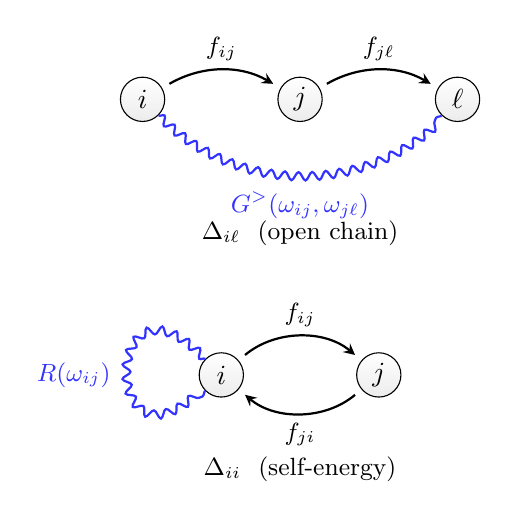
\begin{tikzpicture}[>=stealth, node distance=1.8cm,
      site/.style={circle, draw, top color=white, bottom color=gray!15, inner sep=2pt, minimum size=16pt},
      prop/.style={->, thick, shorten >=3pt, shorten <=3pt}]

    %-- Top panel: open chain (off-diagonal) --%
    \node[site] (i1) at (0,3.5)   {$i$};
    \node[site] (j1) at (2,3.5)   {$j$};
    \node[site] (l1) at (4,3.5)   {$\ell$};
    \draw[prop] (i1) to[bend left=30] node[above,font=\small]{$f_{ij}$} (j1);
    \draw[prop] (j1) to[bend left=30] node[above,font=\small]{$f_{j\ell}$} (l1);
    \draw[decorate, decoration={snake,amplitude=1.5pt,segment length=5pt},
          thick, blue!80] (i1) to[bend right=45] node[below=0.1cm,font=\small]{$G^{>}(\omega_{ij},\omega_{j\ell})$} (l1);
    \node[font=\small] at (2, 1.8) {$\Delta_{i\ell}$ \ (open chain)};

    %-- Bottom panel: self-energy loop (diagonal) --%
    \node[site] (i2) at (1,0)   {$i$};
    \node[site] (j2) at (3,0)   {$j$};
    \draw[prop] (i2) to[bend left=40] node[above,font=\small]{$f_{ij}$} (j2);
    \draw[prop] (j2) to[bend left=40] node[below,font=\small]{$f_{ji}$} (i2);
    \draw[decorate, decoration={snake,amplitude=1.5pt,segment length=5pt},
          thick, blue!80] (i2) .. controls (-0.5, 1.5) and (-0.5, -1.5) .. node[left=0.1cm,font=\small]{$R(\omega_{ij})$} (i2);
    \node[font=\small] at (2, -1.2) {$\Delta_{ii}$ \ (self-energy)};

  \end{tikzpicture}
  \caption{Diagrammatic structure of the influence exponent $\Delta(\beta)$ in the $H_Q$ eigenbasis.
    \textit{Top}: The off-diagonal element $\Delta_{i\ell}$ (open chain) sums intermediate sites $j$,
    weighted by the bath propagator $G^{>}(\omega_{ij},\omega_{j\ell})$ (wavy line) and two coupling
    insertions $f$ (arrows). Energy is not conserved at the intermediate vertex.
    \textit{Bottom}: The diagonal element $\Delta_{ii}$ (self-energy) is a closed loop $i\!\to\!j\!\to\!i$;
    the resonant condition $\omega_1+\omega_2=0$ is satisfied, and the bath propagator collapses to
    $R(\omega_{ij})$.}
  \label{fig:delta_diagrams}
\end{figure}
\subsection{KMS symmetry and the symmetrised reduced state\label{subsec:kms_symmetry}}

The bath kernel $K(\tau)$ satisfies the KMS periodicity condition $K(\tau)=K(\beta-\tau)$,
which in Laplace space reads
\begin{equation}
    \mathcal{K}(-\omega) = e^{-\beta\omega}\,\mathcal{K}(\omega).
    \label{eq:KMS_Klaplace}
\end{equation}
Substituting into the closed form Eq.~\eqref{eq:Ggt_closed_form} and simplifying gives a
corresponding symmetry of the ordered Green function:
\begin{equation}
    G^{>}(-\omega_2,-\omega_1) = e^{-\beta(\omega_1+\omega_2)}\,G^{>}(\omega_1,\omega_2).
    \label{eq:Ggt_KMS}
\end{equation}
Because transition frequencies telescope, $\omega_{ij}+\omega_{j\ell}=\omega_{i\ell}$, applying
Eq.~\eqref{eq:Ggt_KMS} to the matrix-element formula Eq.~\eqref{eq:Delta_matrix_elements}
immediately yields the \emph{detailed-balance} constraint
\begin{equation}
    \Delta_{\ell i} = e^{-\beta\omega_{i\ell}}\,\Delta_{i\ell}^{\ast},
    \label{eq:Delta_detailed_balance}
\end{equation}
or in operator form $\Delta^{\dagger}=\Pi\,\Delta\,\Pi^{-1}$ where $\Pi\equiv e^{-\beta H_Q}$.
Although $\Delta$ itself is not self-adjoint, this relation is a precise constraint: the product
$\Pi\Delta$ is Hermitian.

This symmetry allows us to recast the unnormalised reduced state Eq.~\eqref{eq:rhobar_product} into a manifestly positive, Hermitian form. Writing the bare Gibbs factor as $\Pi \equiv e^{-\beta H_Q}$ gives $\bar\rho_Q = \Pi\,e^{\Delta}$. By splitting $\Pi = \Pi^{1/2}\Pi^{1/2}$ and inserting the identity $\Pi^{-1/2}\Pi^{1/2}=\mathbf{1}$, we symmetrically distribute the bare weight:
\begin{equation}
    \bar\rho_Q
    = \Pi^{1/2} \big( \Pi^{1/2}\,e^{\Delta}\,\Pi^{-1/2} \big) \Pi^{1/2}.
    \label{eq:rhobar_split}
\end{equation}
Applying the operator identity $A\,e^{B}A^{-1} = \exp(A B A^{-1})$ to the inner bracket yields
\begin{equation}
    \bar\rho_Q
    = \Pi^{1/2}\,e^{S}\,\Pi^{1/2},
    \qquad
    S \;\equiv\; \Pi^{1/2}\,\Delta\,\Pi^{-1/2},
    \label{eq:rhobar_symmetric}
\end{equation}
where $S$ is the \emph{symmetrised influence operator}. Its matrix elements evaluate to
$S_{i\ell}=e^{-\beta\omega_{i\ell}/2}\Delta_{i\ell}$, which by Eq.~\eqref{eq:Delta_detailed_balance} satisfy
$S_{i\ell}^{\ast}=S_{\ell i}$. Thus, the modified exponent $S$ is strictly self-adjoint.
The partition function of the reduced system follows by cyclicity of the trace:
\begin{equation}
    Z_Q
    \;\equiv\;
    \operatorname{Tr}[\bar\rho_Q]
    = \operatorname{Tr}[\Pi\,e^{S}]
    = \sum_i e^{-\beta E_i}\,(e^{S})_{ii}.
    \label{eq:ZQ_sym}
\end{equation}
Since $S$ is self-adjoint, $(e^{S})_{ii}\geq e^{S_{ii}}=e^{\Delta_{ii}}$ by Jensen's inequality
applied to the spectral weights $|\langle i|n\rangle|^2$, giving the bound
\begin{equation}
    Z_Q \;\geq\; \sum_i e^{-\beta E_i+\Delta_{ii}},
    \label{eq:ZQ_bound}
\end{equation}
where the right-hand side is a Boltzmann sum with bath-shifted energies and equality holds
when $S$ is diagonal (i.e.\ when $H_Q$ and $\Delta$ share an eigenbasis). The full result
$Z_Q=\operatorname{Tr}[\Pi e^{S}]$ captures all level-mixing corrections through the
off-diagonal elements of $S$.
